\documentclass{article} 
\usepackage{todonotes}
\usepackage{graphicx}
\graphicspath{ {images/} }


\title{URL-Shortener}
\author{Francesco Balzano}


\begin{document}
  \pagenumbering{gobble}
  \maketitle
  \newpage
  \tableofcontents
  \newpage
  \pagenumbering{arabic}
  
\section{Overview}  
URL shortening is the translation of a long Uniform Resource Locator (URL) into an abbreviated alternative that redirects to the longer URL.  A shortened URL may be desired for messaging technologies that limit the number of characters in a message, for reducing the amount of typing required if the reader is copying a URL from a print source, for making it easier for a person to remember, or for the intention of a permalink.\\  
The aim of this project is to provide the implementation of a distributed url-shortener service.


\section{Design choices}
There are three fundamental metrics in the assessment of a distributed system: Consistency, Availability and Partition Tolerance. It is well known from the CAP theorem that it is impossibile to achieve all of them at the same time in a distributed system. \\ 
In this project, I have chosen to focus on availability and partition tolerance, at the expense of consistency. In particular, the consistency model is not a strong one.
In the following subsections, I list and explain the design choices that I made.


\subsection{API}
The url-shortener project is a service that provides the following APIs:

\paragraph{get}
Given the shorten url returns the original url, if present. \\
\texttt{get(shortUrl) -$>$ longUrl}

\paragraph{put}
Generates and returns the shortened url associated with the provided url. \\
\texttt{put(longUrl) -$>$  shortUrl}

\paragraph{remove}
Removes the couple \texttt{<shortened url, original url>}.\\
\texttt{remove(shortUrl) -$>$  longUrl}


\subsection{Passive Replication}
Clients can communicate with every node. If the contacted node is the primary for that request, it will execute the request and directly return the result to the client; otherwise it will forward the request to the primary, which will execute it and send back the response to the sending node, which in turn will hand it back to the client. \\

I have chosen the Passive Replication strategy because I think it should keep lower the number of version conflicts.

\subsection{Data Partitioning}
The partitioning strategy to map objects into nodes is a dynamic one: namely, it is employed Consistent Hashing with virtual nodes. The use of virtual nodes has potentially two advantages: in case of heterogeneous machines we can assign more virtual nodes to the most powerful machines, so that it will be more likely that these machines will handle a bigger number of items. The other advantage concerns homogeneous machines (\texttt{i.e.} machines with similar computational power, bandwidth, storage...). In this case the use of virtual nodes results in a more fair distribution of items among nodes with higher probability. \\ In case of node leave, due for instance to node crash or network partition, the keys asssigned to this node are automatically assigned to another, working node. Since we have replication of data and we use the gossip protocol to detect dead nodes, we are capable to face the leave of one or more nodes without compromising the functioning of the whole system. In other words, availability and partition tolerance are guaranteed.

\subsection{Data Replication}
We want to achieve availability, so an asynchronous replication strategy is adopted. Namely, the primary node immediately answers to the client after an operation is performed. Messages to the backup nodes are sent periodically, and not after every update of the primary's data. This strategy reduces the latency of the communication client-primary, again at the expense of consistency. \\
Each primary node is associated 1 backup node, which is the next node clockwise in the ring. Every time a primary wishes to update its replica, it sends all the content of its database to this node. 

\subsection{Primary Failure}
The use of Consistent Hashing and the the specific data replication strategy adopted (backup is the next node clockwise in the ring) allows to have a vry easy failover procedure: if node \textit{i} is down, the space of keys that belonged to node \textit{i} will be automatically mapped to node \textit{(i+1) mod n}. Since node \textit{(i+1) mod n} is the backup of node \textit{i} it will have a copy of the keys of node \textit{i} (although possibly not updated), so the correct behaviour will be maintained also in case of failure of the primary without needing an explicit failover procedure. For further details about the failover procedure please refer to the  \textit{Implementation} section.    


\subsection{Consistency Model}
This project adopts an eventual consistency model. \todo{In realtà tutte le richieste arrivano a un leader}It is possible to get different results if running the same query at the same time on the leader and on a follower. This may happen if the follower has an outdated version of the leader's data. Anyway this is only a temporary state: if we stop writing to the database for a while, the followers will eventually become consistent with the leader. I decided to accept this weak consistency model in order to have better availability and partition tolerance. 

\subsection{Conflicts Resolution}
Each node is assigned a vector clock that allows it to order events, that is to track causal dependencies between events. When a message is sent from a node to another, it carries both the object (the target of the communication) and the sender's vector clock. If the recipient node already has that object with the associated vector clock in its database, two situations may arise:
\begin{itemize}
\item  If one vector clock is smaller than the other, keep the greatest (i.e. latest) version of the object;
\item  \todo{Non ti puoi affidare al client per risolvere inconsistenze, va fatto server-side}If that is not the case, the two vector clocks are concurrent, and if the two objects are assigned different values then we have a conflict.
\end{itemize}



\section{Implementation}  
There are clients, that invoke the service, and nodes, that comprise the cluster and actually implements the service. Clients and nodes stay in two different modules: the formers in the client module, the latters in the core module. Indeed they are logically different things, and so they should be able to evolve independently from each other. 

\subsection{Architecture} 

The client can make a request to any node in the cluster. The nodes process the request and handle back the result to the client. \todo{Molto specifico, inseriscilo negli use cases?} In particular, only the primary node for a given request actually processes it. If a node receives a request for which it is not the primary, it discovers who is the primary and forwards the request to such node. The primary node processes the request and then handles back the result to the previous node, who in turn returns the response to the client. \\
Each node has to do three main jobs, so I created a node as a container of three services: 
\begin{itemize}
\item \textit{client communication service}: each node must be able to communicate with the client, to accept requests from it and return responses;
\item \textit{node communication service}: each node must be able to communicate with the other nodes. Indeed, it could have to forward the client request to the primary node, or to send the content of its own database to the backup node, or even only to check that the other nodes of the cluster are alive;
\item \textit{storage service}: each node must have a database, to store and retrieve urls on client's behalf. Actually, it has two databases: its own database, used to handle requests, and the backup database, used to replicate the data of another node+.
\end{itemize}

\begin{figure}[h]
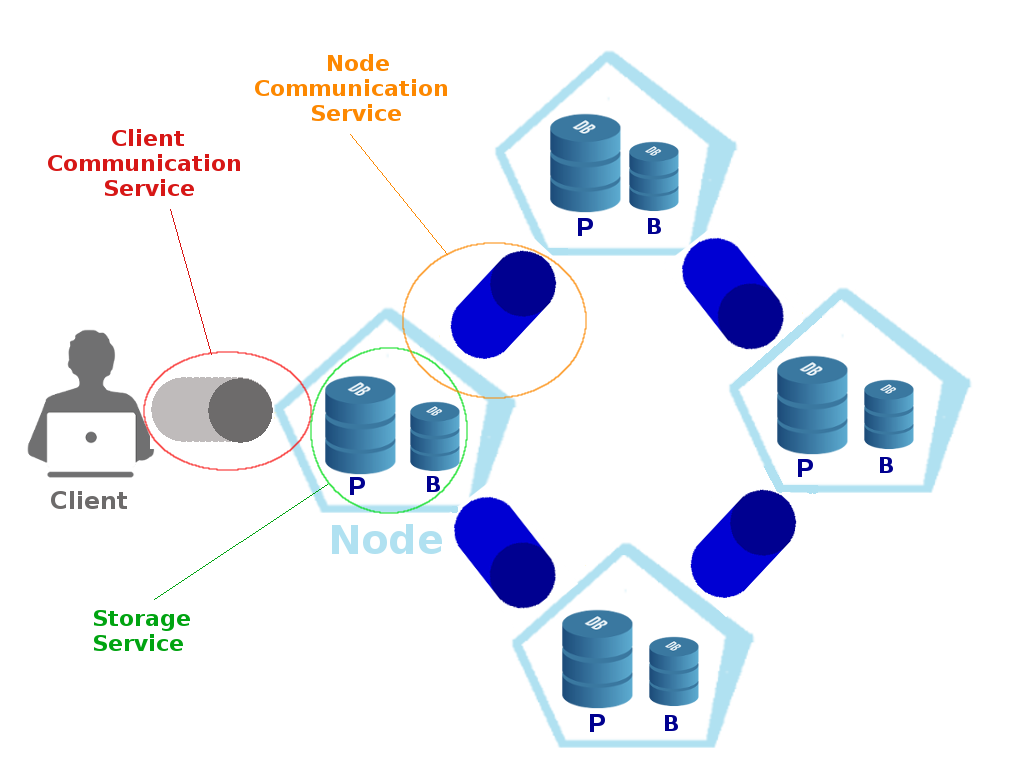
\includegraphics[scale=0.35]{architecture}
\caption{General architecture. There is a client and a cluster, which is made of more nodes. Each node is made of a node communication service, a client communication service and a storage service. The letter ``P'' under the database stays for ``primary'' , the letter ``B'' for ``backup''.}
\end{figure}

\subsection{The project classes} 
The structure of the project is the following. The node is the building block of the cluster and, as we already said, it is made of three main \textit{services}. Each of these services provides a high level view of the functionalities it has to implement. For the actual implementation the managers rely on proper \textit{managers}, which have the responsability to setup things and handle lower level details. The following figure shows a simplified UML class diagram, in which the relationships among classes are highlighted (but not the methods).

\subsubsection{The core module} 

\subsubsection{The client module} 

\subsection{Use cases} 

\subsubsection{Management of a client request} 

\subsubsection{Replication of data} 

\section{Test}

\subsubsection{Correct behaviour of put, get, remove} 

\subsubsection{Self-healing } 
\todo[inline]{ (Primary failure) Show that in case of primary failure the system still works correctly, without needing any manual intervention}


\subsubsection{Conflict Resolution} 

\subsubsection{Load Balancing} 
\todo[inline]{Tweak the number of virtual nodes to show that more powerful machines can actually be assigned more items} 


\section{Future work} 
\begin{itemize}
\item Hash function for the url shortener. \todo[inline]{32 bit hash function allows too few urls; and in that case find another method to translate sequence of bytes into allowed charactes [A-Za-z0-9]}
\end{itemize}

\end{document}
